\documentclass[10pt, letterpaper]{article}

\usepackage{amssymb,amsmath,amsfonts,eurosym,geometry,ulem,graphicx,caption,color,setspace,sectsty,comment,footmisc,caption,natbib,pdflscape,subfigure,array,hyperref}
\usepackage{xcolor}
\usepackage{mathptmx}
\usepackage{listings}
\lstset{language=Matlab}
\hypersetup{
    colorlinks,
    linkcolor={red!50!black},
    citecolor={blue!50!black},
    urlcolor={blue!80!black}
}
\normalem
\usepackage[flushleft]{threeparttable}
    
\onehalfspacing
\newtheorem{theorem}{Theorem}
\newtheorem{corollary}[theorem]{Corollary}
\newtheorem{proposition}{Proposition}
\newenvironment{proof}[1][Proof]{\noindent\textbf{#1.} }{\ \rule{0.5em}{0.5em}}

\newtheorem{hyp}{Hypothesis}
\newtheorem{subhyp}{Hypothesis}[hyp]
\newtheorem{asu}{Assumption}
\renewcommand{\thesubhyp}{\thehyp\alph{subhyp}}

\newcommand{\red}[1]{{\color{red} #1}}
\newcommand{\blue}[1]{{\color{blue} #1}}

\newcolumntype{L}[1]{>{\raggedright\let\newline\\arraybackslash\hspace{0pt}}m{#1}}
\newcolumntype{C}[1]{>{\centering\let\newline\\arraybackslash\hspace{0pt}}m{#1}}
\newcolumntype{R}[1]{>{\raggedleft\let\newline\\arraybackslash\hspace{0pt}}m{#1}}

\geometry{left=1.0in,right=1.0in,top=1.0in,bottom=1.0in}

\begin{document}

\title{Homework 1: ECON512}
\author{Joonkyo Hong}
\date{}
\maketitle
\smallskip

\noindent The relevant state variables are $(s,p)$, where $s$ is the remaining amounts of trees today and $p$ is the today's price. The control variable is $s'$: the remaining amounts of trees tomorrow.

Thus, the relevant Bellman equation is as follow:
\begin{align*}
V(s,p) & = p(s-s') - 0.2(s-s')^{1.5} + \delta E_{p'|p} V(s',p') \\
       & = p(s-s') - 0.2(s-s')^{1.5} + \delta \sum_{p'} V(s',p')\pi(p'|p), 
\end{align*}
where $\pi(p'|p)$ is a transition probability of future state being $p'$ given that current state is $p$.

The results from solving the above Bellman equation with grids 21 for $p$ are displayed in Figure 1. As the initial amounts of tree increase, the value of a firm also increases no matter what the lumber price is. When the initial amounts are fixed, then the value of a firm increases in the lumber price. I report the optimal harvest amounts as a function of the current remaining amounts of tree. Given the lumber price, the optimal harvest policy function is increasing in the current stock. That is, if a firm has more stocks at the beginning of the period, a firm would like to harvest more. Furthermore, given the current remaining amounts of tree, a firm would like harvest more as the lumber price increases.

The results with five grids are reported in Figure 2. Though there are some discrepancies with the functions that I obtained with 21 grids, the qualitative interpretation remains unchanged.

Finally, Figure 3 is displaying the 20 period-trajectory of the remaining amounts of tree when a firm has 100 trees and faces $p=1$ at the initial state. The solid line is displaying the predicted values and the dashed lines are displaying 90\% confidence interval. To compute this trajectory, I follow the algorithm below:\\

\noindent [1] Let $\bold{s} = (s,p)$, and compute the relevant Markov transition probability ${\mathcal P}$.

\noindent [2] Start with the initial probability $\bar{\pi}$ whose value is 1 if the array is corresponding to $\bold{s} = (100,1)$, and 0 otherwise.

\noindent [3] For $k=1,2,\cdots,20$, compute $\bar{\pi}^{k}=\bar{\pi} {\mathcal P}^{k}$, and generate the distribution of $s$, namely $f_{s}^{k}$. 

\noindent [4] Store 5\%-quantile, mean, and 95\%-quantile for each $k=1,2,\cdots,20$.\\

 Since there is no growth in the remaining amounts of trees in this model, it would not be surprising that the remaining amounts of tree would go to zero in the future.
 
\begin{figure}
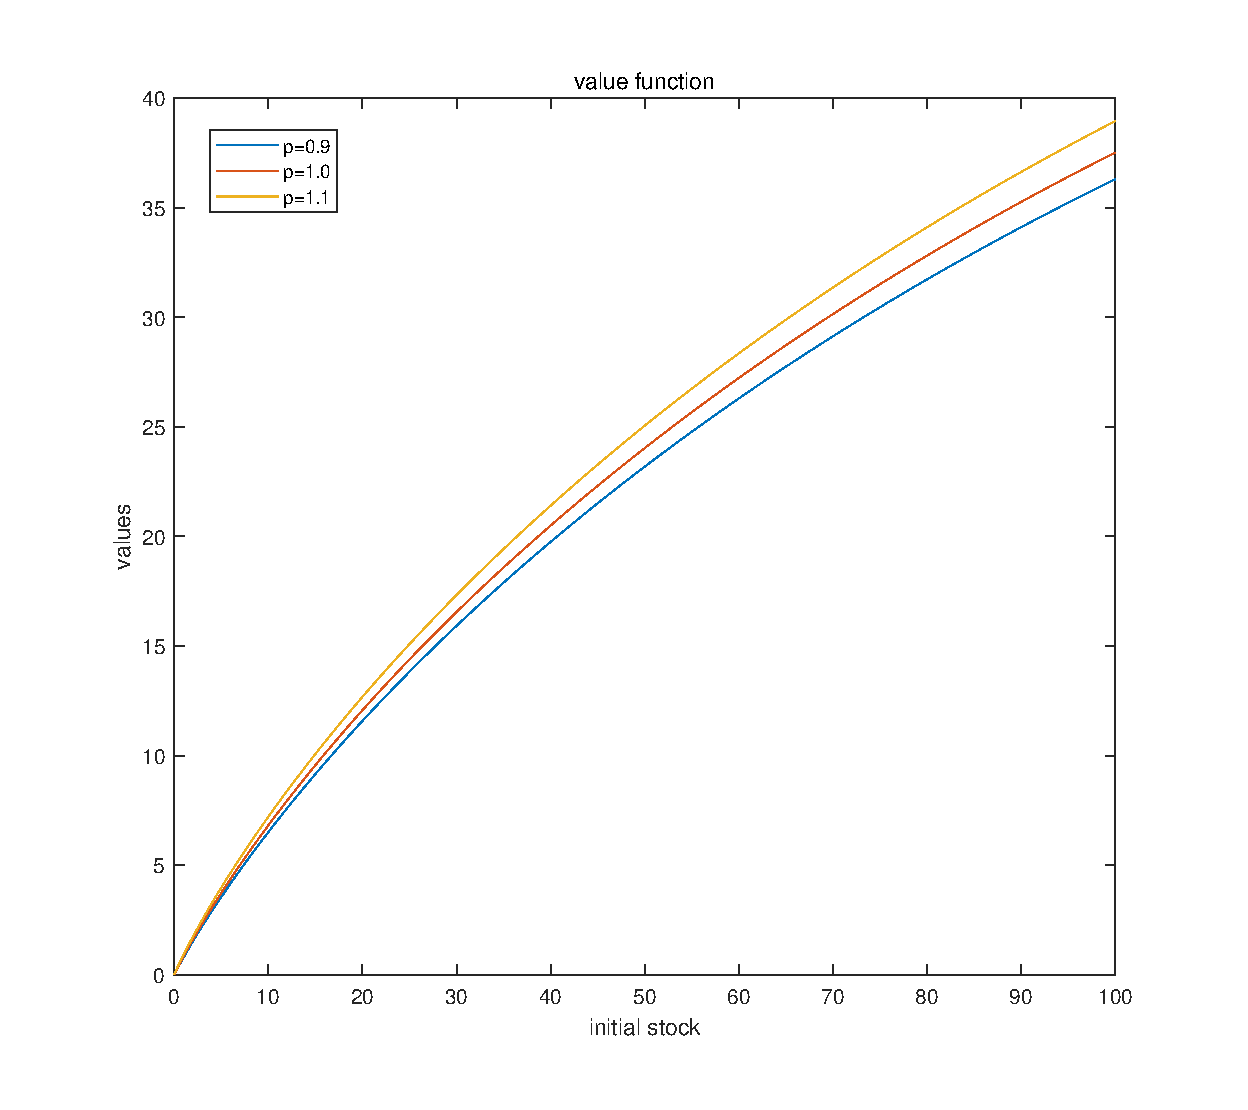
\includegraphics[width=0.5\textwidth]{value_grid21.eps}
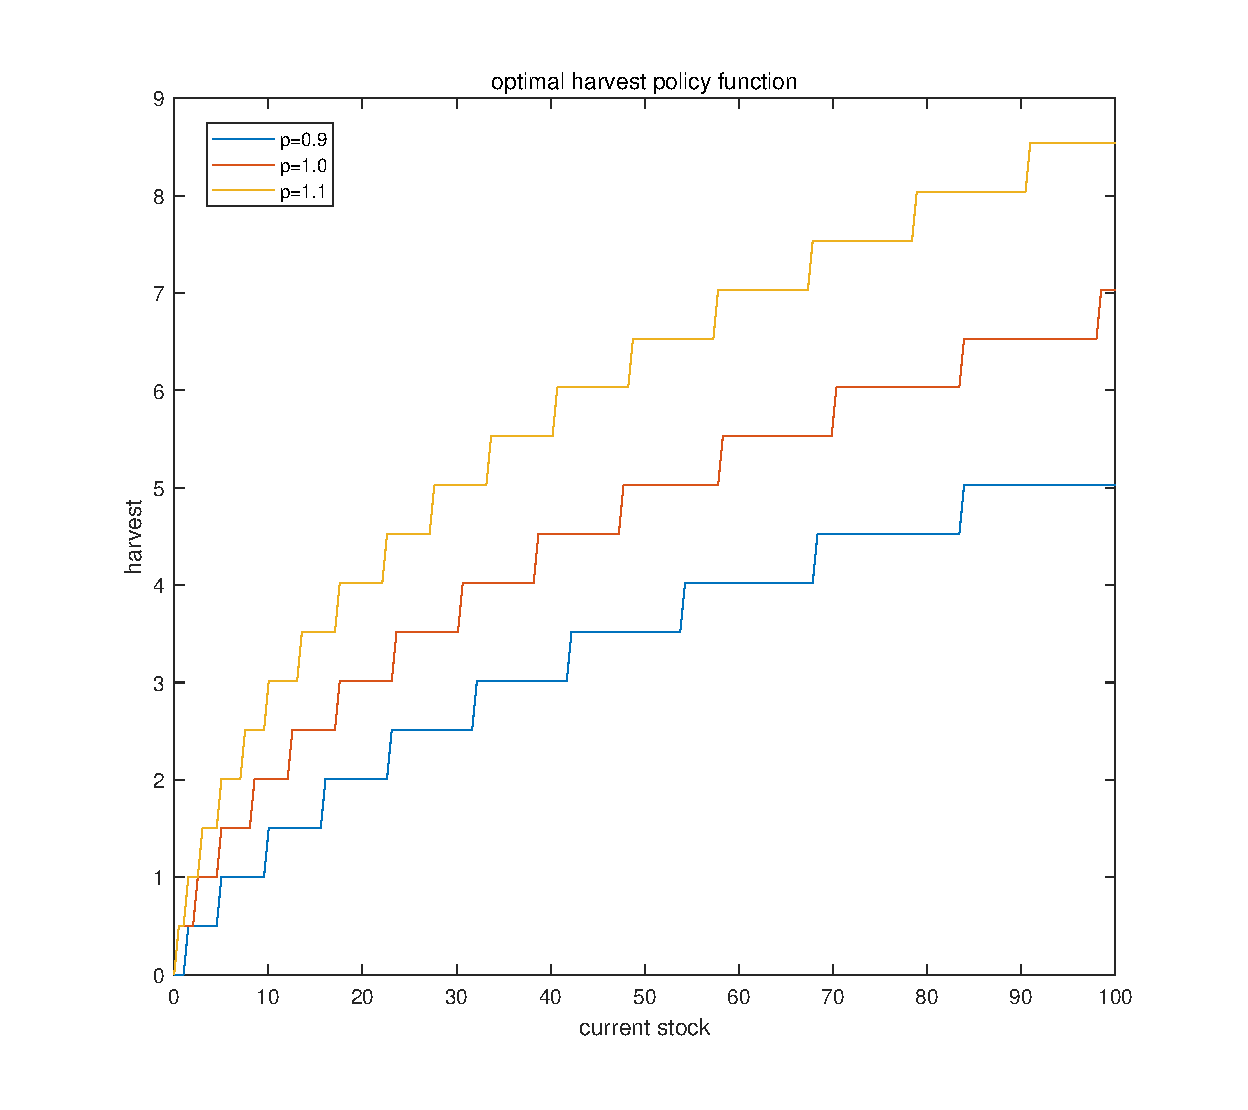
\includegraphics[width=0.5\textwidth]{policy_grid21.eps}
\caption{Results with 21 Grids}
\end{figure}



\begin{figure}
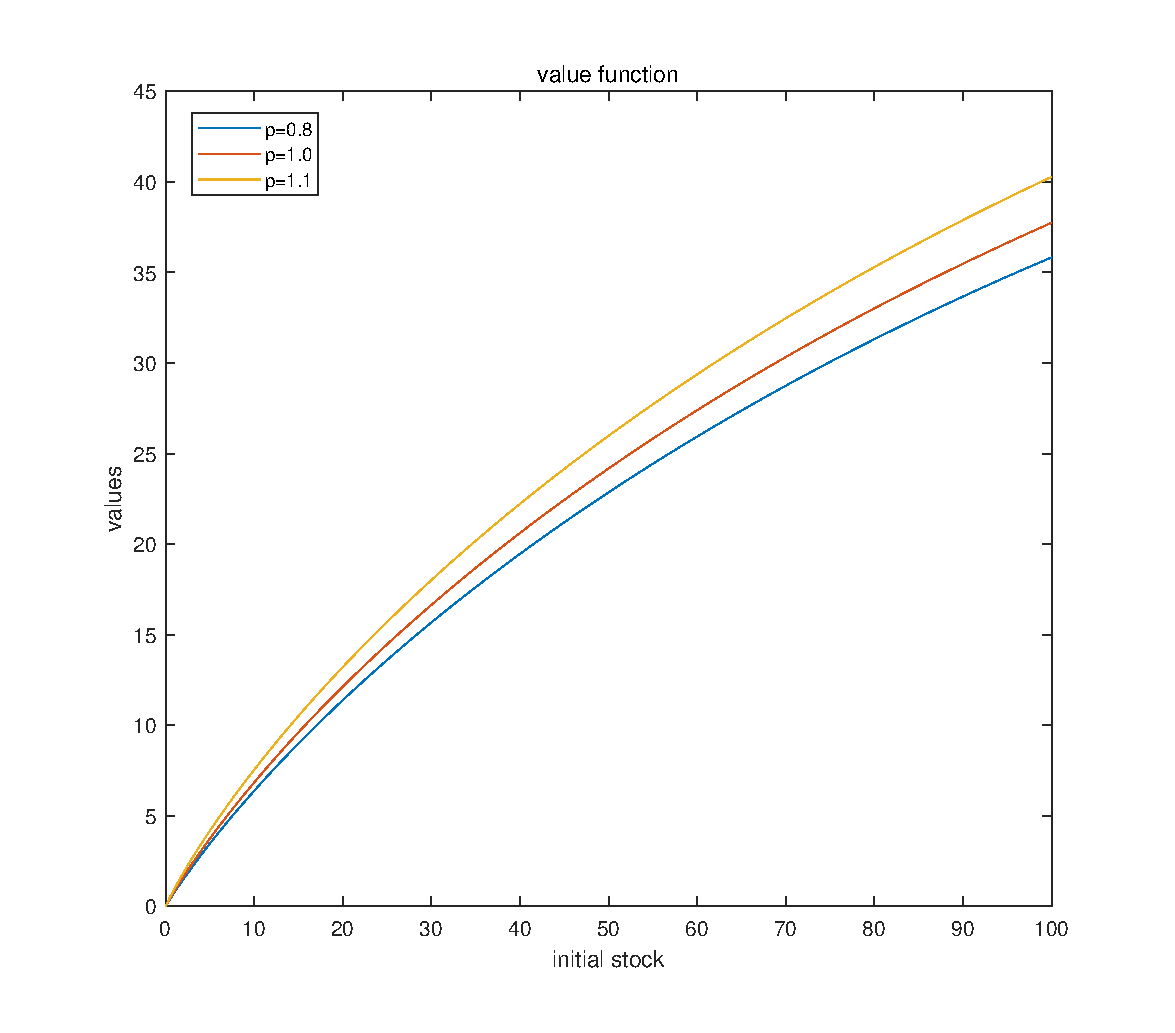
\includegraphics[width=0.5\textwidth]{value_grid5.eps}
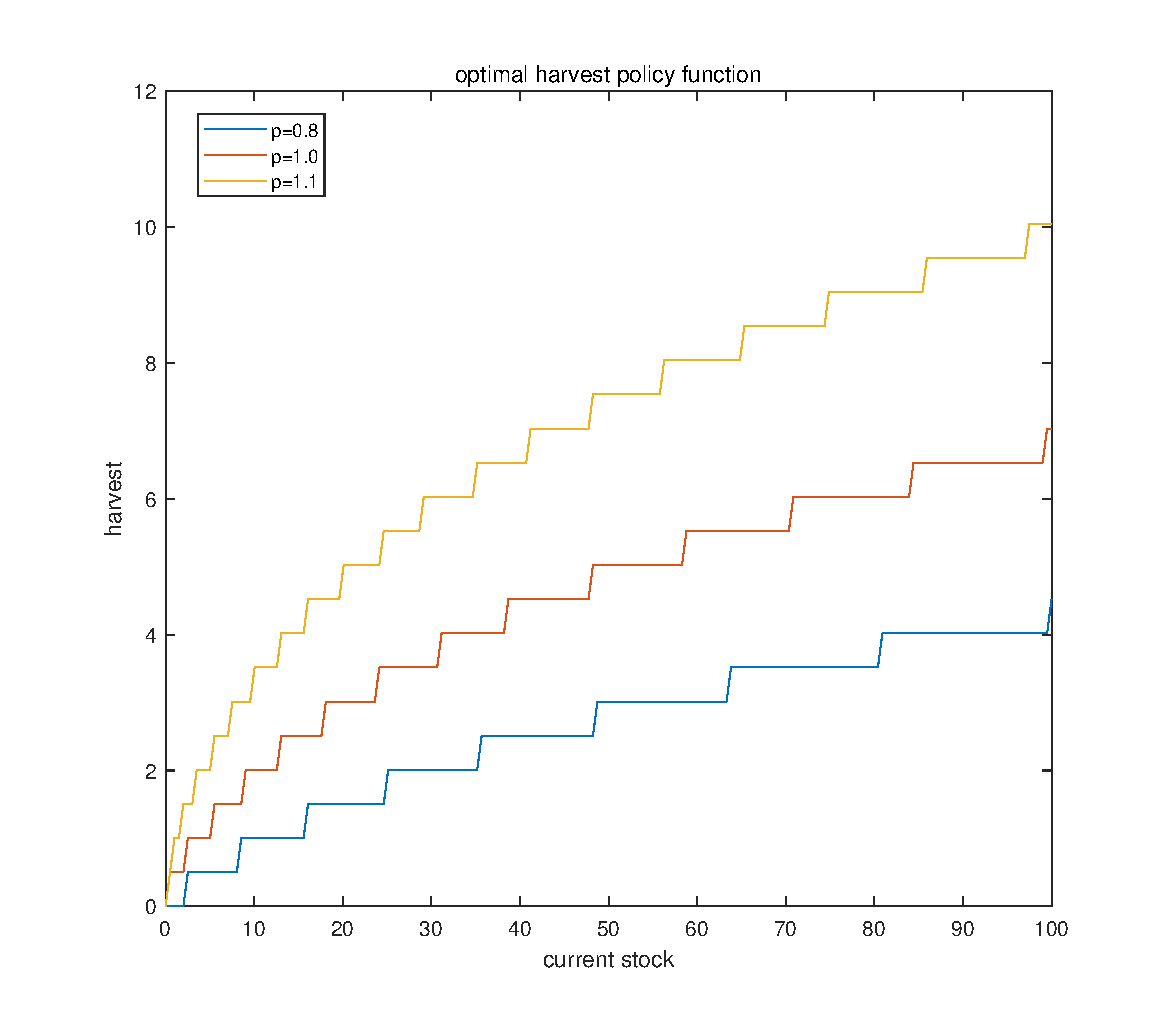
\includegraphics[width=0.5\textwidth]{policy_grid5.eps}
\caption{Results with 5 Grids}
\end{figure}

\begin{figure}
\centering
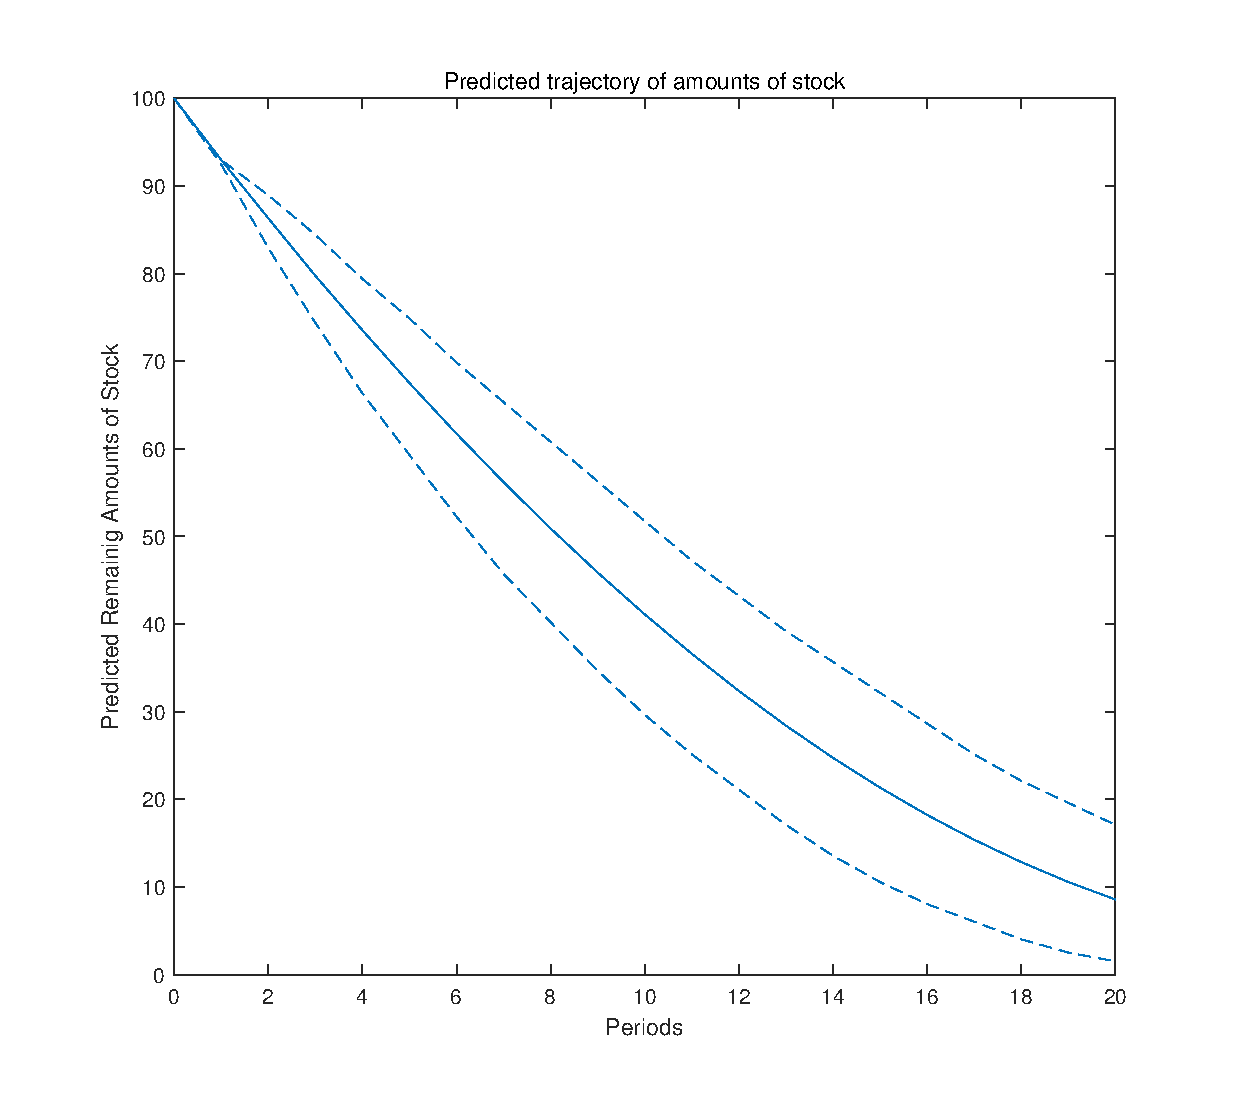
\includegraphics[width=0.6\textwidth]{trajectory_grid21.eps}
\caption{Trajectory of the Remaining Amounts of Tree}
\end{figure}


\clearpage

\begin{verbatim}
%%%%%%%%%%%%%%%%%%%%%%%%%%%%%%%%%%%%%%%%%%%%%%%%%%%%%%%%%%%
% Homework #5 ECON 512                                    %
% Written by Joonkyo (Jay) Hong, 18 Nov 2018              %
%%%%%%%%%%%%%%%%%%%%%%%%%%%%%%%%%%%%%%%%%%%%%%%%%%%%%%%%%%%
% Code for HW1 ECON512
% Written by Joonkyo Hong
% Build upon stochgrow.m in ECON512 lecture
% Jan 23, 2019


%% Section 1. Solve for Value functions

% Parameter values

 delta=0.95; % discount factor
  
 Z=21;          % grid number for shocks
 sigma=0.1;     % std of error term in AR(1) process
 mu=0.5;        % unconditional mean 
 ro=0.5;        % AR(1) parameter 
 
 

% GRID FOR STOCK

N=200;

s0 = 100;              % Initial value of stock 
slow = 0;    % In the end, the stock will be zero because there's no growth
grids = ((s0)-slow)/(N-1);
s = slow:(grids):(s0);

% GRID FOR PRICE PROCESS

% grid for shock by using Tauchen's method for finite state Markov
% approximation

[prob,grid]=tauchen(Z,mu,ro,sigma);
disp(['The dimensions of prob are ' num2str(size(prob)) ])
disp(['The dimensions of grid are ' num2str(size(grid)) ])

% VALUE FUNCTION ITERATION

vinitial=zeros(N,Z);
vrevised=zeros(N,Z);
decision=zeros(N,Z);
  
invest=kron(ones(1,Z),s');
disp(['The dimensions of invest  are ' num2str(size(invest)) ])
ONE=ones(N,1);
 
%iteration

diff=1;

while diff>0.001
    
    Ev=vinitial*prob';   % find the expected value of value function
      
    for i=1:N           % for each k, find the optimal decision rule
      pi = profit(s(i),s,grid);  
      [vrevised(i,:),decision(i,:)]=max(pi+delta*Ev);
    end
    
     diff=norm(vrevised-vinitial)/norm(vrevised)
     vinitial=vrevised;
    
end

% compute decision rule

derule=zeros(N,Z);

for j=1:Z
    derule(:,j)=s(decision(:,j))';
end

net_invest = kron(ones(1,Z),s') - derule;

figure(1)
plot(s,[vrevised(:,8) vrevised(:,11) vrevised(:,14)]);
xlabel('initial stock');
ylabel('values');
title('value function');


figure(2)
plot(s, [net_invest(:,8) net_invest(:,11) net_invest(:,14)]);
xlabel('current stock');
ylabel('harvest');
title('optimal harvest policy function');


%% Section 2. Predicting remaining amounts of stock

% Compute the transition probability of state

     P=zeros(Z*N,Z*N);

     for i=1:Z
         for j=1:Z
              P((i-1)*N+1:i*N,(j-1)*N+1:j*N)=prob(i,j)*(kron(ones(1,N),derule(:,i))==kron(ones(N,1),s));
        
         end
     end
     

% Initial probability for the state with stock 100 and price 1

    index_1 = find(grid==1);
    pinitial = zeros(1,N*Z);
    pinitial(1,index_1*N)=1;
    
    
% Simulate the model

    tau = 20;           % # of Periods for expectation
    predicted = zeros(tau,3);
    
    
   for t=1:20
       
       px = pinitial*P;
       probs=zeros(N,Z);
       
       for i=1:Z
           probs(:,i) = px((i-1)*N+1:i*N)';
       end
       
       probs = sum(probs');
       cdf = cumsum(probs);
       lower = max(find(cdf<=0.05));
       upper = min(find(cdf>=0.95));
       
       mean = probs*s';
       lowerbdd = s(lower);
       upperbdd = s(upper);
       
      predicted(t,:) = [lowerbdd mean upperbdd];
      
    
   pinitial = px;
      
   end
   
       
figure(3)
plot(0:1:20, [100 100 100;predicted]);
xlabel('Periods');
ylabel('Predicted Remainig Amounts of Stock');
title('Predicted trajectory of amounts of stock');

\end{verbatim}
                     

\end{document}